\documentclass[10pt,a4paper]{book}
\usepackage[utf8x]{inputenc}
\usepackage{ucs}
\usepackage{amsmath}
\usepackage{amsfonts}
\usepackage{graphicx}
\makeatletter
\def\ScaleIfNeeded{%
\ifdim\Gin@nat@width>\linewidth
\linewidth
\else
\Gin@nat@width
\fi
}
\makeatother
\usepackage[bookmarksnumbered=true,bookmarksopen=true]{hyperref}
\author{Christian Brandt & Florian Thomas}
\title{Entwicklung webbasierter Software}
\date{Wintersemester 2011/2012}
\begin{document}
\begin{titlepage}
\begin{center}
\LARGE{Technische Hochschule Mittelhessen}
\linebreak
\large{Fachbereich MNI - Mathematik, Naturwissenschaften \& Informatik}
\linebreak 
\linebreak
\linebreak
\linebreak
\linebreak
\linebreak
\linebreak
\LARGE{Entwicklung webbasierter Software}
\linebreak
\linebreak
\linebreak
\linebreak
\linebreak
\linebreak
\linebreak
\large{Prüfer}
\linebreak
\large{MSc. Martin Karry}
\linebreak
\linebreak
\large{Prüflinge}
\linebreak
\large{Christian Brandt \& Florian Thomas}
\linebreak
\linebreak
\linebreak
\linebreak
\Large{Projekt: Treebook}
\linebreak
\normalsize{Ein soziales Netzwerk mit Anbindung an Facebook und flickr}
\linebreak
\linebreak
\linebreak
\linebreak
\linebreak
\linebreak
\normalsize{Wintersemester 2011/2012}
\end{center}
\end{titlepage}
\setcounter{page}{1}
\subsubsection{Eidesstattliche Erklärung}

\tableofcontents
\renewcommand{\chaptername}{}
\renewcommand{\thechapter}{}
\renewcommand{\thesection}{\arabic{section}}
\renewcommand{\thefigure}{\arabic{figure}}

\chapter{Einleitung}
Im Rahmen der Veranstaltung "Entwicklung webbasierter Software", geleitet von Herrn MSc. Martin Karry, soll zum Bestehen eine webbasierte Software entwickelt werden.
\chapter{Einführung}
Die hier beschriebene Software ist ein soziales Netzwerk, vergleichbar mit Facebook\footnote{\href{http://facebook.com/}{http://facebook.com/}} oder Google+\footnote{\href{http://plus.google.com/}{http://plus.google.com/}}. Der Name "Treebook" leitet sich aus der Struktur der Freundschaften innerhalb dieser Software her. Dieses System ist angelehnt an das Circle-System von Google+\footnote{\href{http://www.youtube.com/watch?v=BeMZP-oyOII}{http://www.youtube.com/watch?v=BeMZP-oyOII}}: Der Benutzer (Baum) besitzt mehrere "Trees" (Äste) in denen wiederum mehrere Benutzer enthalten sein können.

Treebook benutzt mehrere Application programming interfaces (nachfolgend kurz API) um die Funktionsmöglichkeiten der Software zu erweitern. Dem Benutzer ist es so mit Hilfe der API von Facebook möglich, sich mit seinen Facebook-Zugangsdaten bei Treebook anzumelden. Die API des Bilderdienstes Flickr\footnote{\href{http://flickr.com}{http://flickr.com}} wird verwendet um dem Anwender zu ermöglichen innerhalb von Treebook mit seinen auf Flickr bereitgestellten Fotos zu interagieren (Fotos ansehen, kommentieren, hochladen).

Der Anwender hat mehrere für ein soziales Netzwerk typische Aktionen zur Auswahl. Er kann Nachrichten (sogenannte "Posts") schreiben, die er mit von ihm ausgewählten "Trees" teilt. Leser einer Nachricht können diese kommentieren, mögen und im Gegensatz zu den bekannten sozialen Netzwerken auch Ablehnung zeigen.

Dem Benutzer steht ein eigenes Profil zur Verfügung in dem er Informationen über sich für die anderen Benutzer veröffentlichen kann. Diese Informationen sowie eventuelle Fotos können über die Privatsphäreneinstellung entweder mit allen angemeldeten Benutzern geteilt werden oder nur mit den eigenen Trees.
\chapter{Analyse}

\chapter{Backend}

\chapter{Frontend}
\section{Allgemeiner Aufbau}
Die Anwendung wird generell in mehreren Schritten geladen. Serverseitig wird zunächst das HTML-Grundgerüst zur Verfügung gestellt, in das nach und nach die gewünschten Inhalte geladen werden.
Dies ermöglichen verschiedene JavaScript-Funktionen, welche neue Informationen per "Asynchronous JavaScript and XML" (kurz AJAX) vom Server abrufen.
Wann und welche Informationen genau vom Server bereitgestellt werden, wird in den folgenden Abschnitten erläutert.

\section{Der Anwendungsstart}
Im Allgemeinen wird beim ersten Besuch der Treebook-Seite die Startseite mit dem Treebook-Logo angezeigt.
\begin{figure}[htbp]
\centering
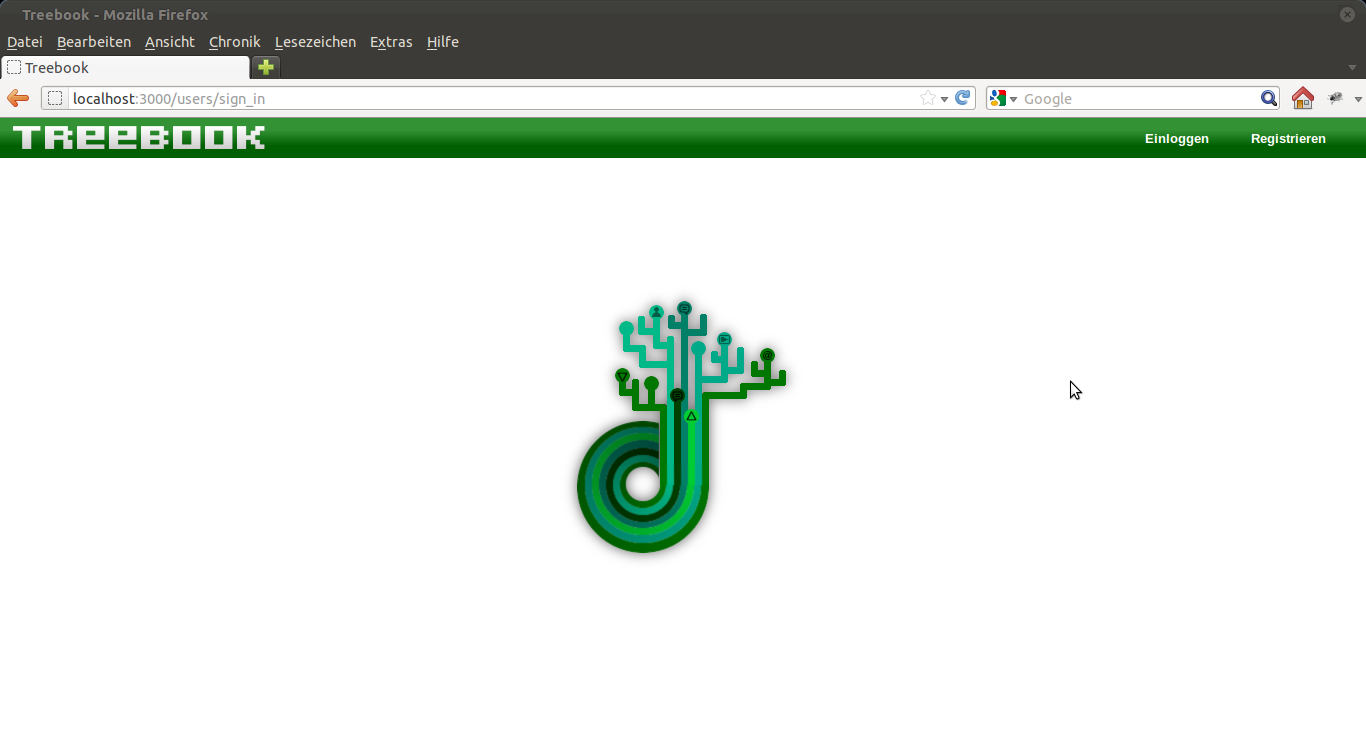
\includegraphics[width=\ScaleIfNeeded]{Pictures/screen_startup.png}%
\caption{Startseite}%
\end{figure}
Von hier aus hat der Anwender die Möglichkeit sich im System anzumelden oder zu registrieren.
Die Anmeldung erfolgt wahlweise über eine dem System bekannte E-Mail-Adresse und dem dazugehörigen Passwort oder über die Facebook-OAuth-API ("Via Facebook anmelden").
Ist der Nutzer dem System noch nicht bekannt, kann er sich dennoch direkt via Facebook anmelden. In diesem Fall wird für ihn ein neues Treebook-Nutzerkonto mit seinen bei Facebook hinterlegten Daten angelegt.

\section{Nach dem Login}
\subsection{Der Stream}
Nachdem sich der Anwender angemeldet hat, sieht er zunächst den sogenannten \textbf{Stream} vor sich. Links davon befindet sich die allgemeine \textbf{Navigation} mit seinen erstellten Trees. Rechts befindet sich ein Suchfeld.
\begin{figure}[htbp]
\centering
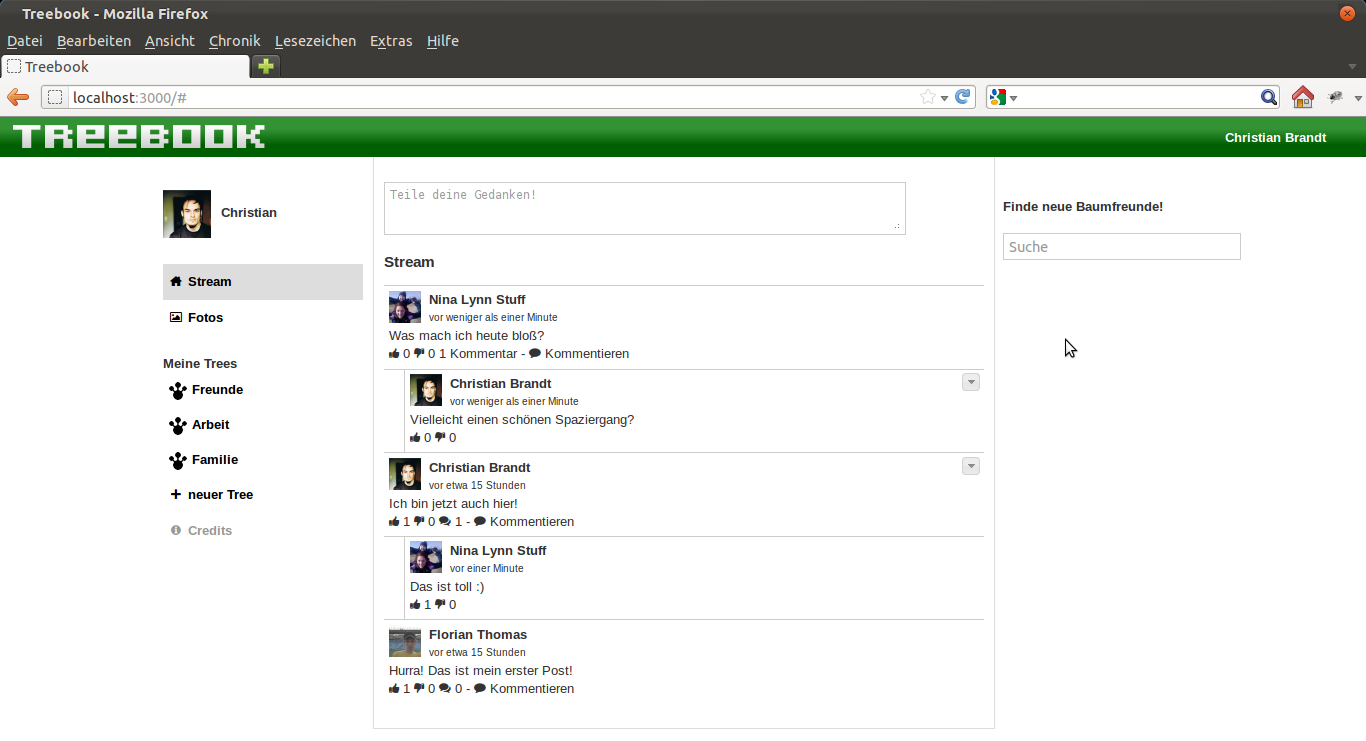
\includegraphics[width=\ScaleIfNeeded]{Pictures/screen_stream.png}%
\caption{Stream}%
\end{figure}
Im Stream werden alle \textbf{Posts} angezeigt, die der Anwender selbst, oder Kontakte in seinen Trees erfasst haben. Diese sind rückwärts sortiert nach Erstellungsdatum, sodass der Anwender am Seitenanfang immer die neuesten Posts sieht und, je weiter er nach unten scrollt, die Posts immer älter werden.
Unter jedem Post werden (sofern vorhanden) die letzten 3 \textbf{Kommentare} zu diesem Post angezeigt. Sind mehr als 3 Kommentare verfügbar, sieht der Anwender einen Link "Alle vorherigen Kommentare anzeigen", welcher nach einem Klick die übrigen Kommentare zum Post anzeigt.
\subsection{Die Navigation}
Die Navigation teilt sich in 4 Unterbereiche auf:
\begin{list}{$\bullet$}{}
\item Das \textbf{Profilbild} und der Vorname des derzeit eingeloggten Nutzers
\item Allgemeine Links zum Stream und zu den \textbf{Fotos} des eingeloggten Nutzers
\item Die vom Nutzer erstellten Trees und ein Link zum Erstellen eines neuen Trees
\item Ein Link zu den \textbf{Credits}
\end{list}
Per Klick auf das Profilbild oder den Vornamen des Anwenders wird das Profil geladen. Standardmäßig sieht der Anwender dann seine eigenen Beiträge aufgelistet.

Mit einem Klick auf "Fotos" wird ebenfalls das Profil des Nutzers geladen, allerdings wird direkt der Foto-Reiter aktiviert.

Klickt der Nutzer auf einen \textbf{Tree}, so werden nur Beiträge angezeigt, die diesem Tree zugeordnet sind, also Beiträge, die vom User explizit für diesen Tree freigegeben wurden, oder Beiträge von Kontakten, die der Nutzer diesem Tree zugeordnet hat.

Ein Klick auf "neuer Tree" zeigt ein Textfeld, in das der Nutzer eine Bezeichnung für den Tree eingibt und zwei Buttons zum Speichern oder Verwerfen des neuen Trees.

Hinter den \textbf{Credits} verbergen sich Links zu Software und sonstigen Ressourcen, die für die Entwicklung von Treebook verwendet wurden.
\chapter{Fazit}

\chapter{Literatur}
\end{document}